%Chapter{Sintesis de óxido de grafeno}
El método de síntesis utilizado está basado en el propuesto por Hummers para la síntesis de óxido de grafito \citep{Hummers1958}, y es descrito por Abdolhosseinzadeh \citep{Abdolhosseinzadeh2015}, la principal diferencia con el procedimiento original de Hummers, es la introducción de etapas de sonicación para asistir en la exfoliación del óxido de grafito.

\section{Procedimiento experimental}
En una síntesis normal 1 g de grafito en polvo (Sigma-Aldrich $>$99\%) o en hojuelas (Superior Graphite $>$80\%), tal como viene envasado, se añaden a 50 ml de ácido sulfúrico (\ce{H_2SO_4}, Baker 97.8\%) en un vaso precipitado de 250 ml previamente puesto en un baño de hielo sobre un agitador magnético, la mezcla se deja agitar por 5 minutos. Una vez el grafito se ha dispersado en el ácido sulfúrico se agregan 3 g de permanganato de potasio (\ce{KMnO_4}, Chemix 99.44\%), lentamente, manteniendo la temperatura de la mezcla bajo los 10 C y así evitar la explosión del permanganato. Luego de 15 minutos de agitación, se quita del baño de hielo y se agita 25 minutos más a temperatura ambiente, seguido de 5 minutos en un baño ultrasónico (99\% de potencia, SB-3200DTD Ultrasonic Cleaner), este proceso de agitación-sonicación es repetido 12 veces, tomando un total de 6 horas en completarse. Una vez completado este proceso, se agregan 200 ml de agua destilada rápidamente, esto produce una reacción exotérmica con evolución de gases, la solución se vuelve marrón, color característico del óxido de grafeno. En general, la solución se divide en dos partes iguales, y se vuelven a sonicar por dos horas más, una de las partes es reducida posteriormente, mientras que la otra se trata con agua oxigenada (\ce{H_{2}O_2}) tal como lo menciona Hummers en su escrito original, para reducir el permanganato y dióxido de manganato restante en la solución \citep{Hummers1958}, 20 ml de \ce{H_2O_2} al 30\% se añaden lentamente mientras se continúa la  agitación, la solución se vuelve de color amarillo brillante al agregar el peróxido de hidrógeno y libera gases. Cuando la evolución de gases cesa, se remueve del agitador magnético y se deja a temperatura ambiente, transcurrido un día de reposo, el material precipita al fondo del vaso, y se procede a remover el resto de la solución acuosa que contiene restos de la reacción para luego rellenar el vaso con agua destilada, este proceso de lavado es realizado al menos cuatro veces y por último se remueve la mayor cantidad de agua, para dejarlo secar a temperatura ambiente.

\section{Resultados}
Del proceso de síntesis anterior se obtienen dos resultados, el óxido de grafeno lavado con peróxido de hidrógeno y lavado, y otro sin lavar que es utilizado para su posterior reducción.

El óxido de grafeno lavado con \ce{H_{2}O_2} es de color marrón claro y una vez seco se oscurece con el pasar de los días.

\begin{figure}
	\centering
	\fbox{
		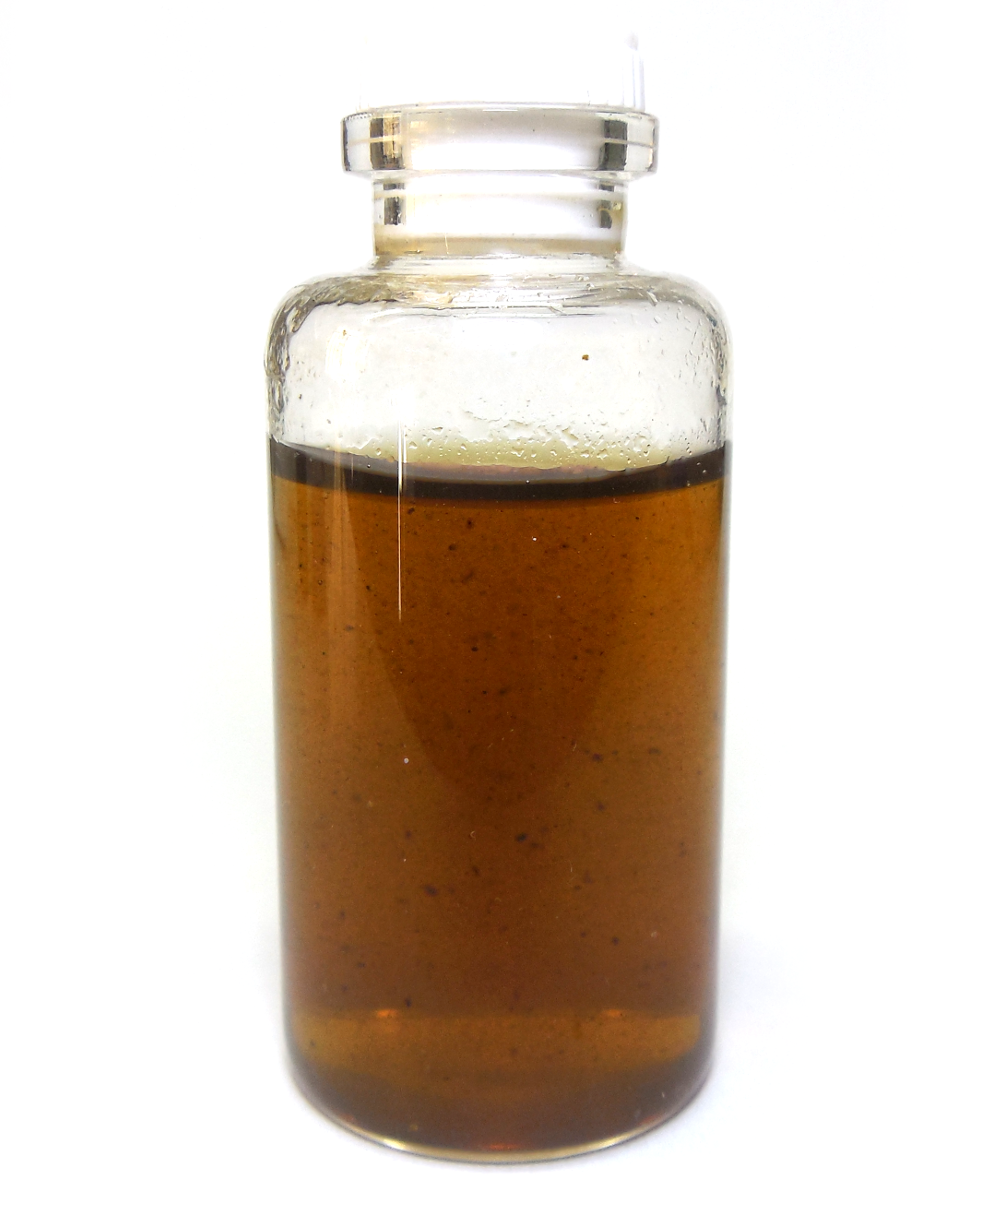
\includegraphics[width=0.5\textwidth]{GO_pic.png}
	}
	\caption{GO}
	\label{fig:GO}
\end{figure}

El óxido de grafeno es caracterizado por espectroscopía de rayos x (XRD), UV-Vis, y microscopia SEM.
